%!TeX root=../tese.tex
%("dica" para o editor de texto: este arquivo é parte de um documento maior)
% para saber mais: https://tex.stackexchange.com/q/78101/183146

%% ------------------------------------------------------------------------- %%
\chapter{Link-Cut Tree}
\label{cap:link-cut-trees}

Neste capítulo, apresentaremos a estrutura de dados link-cut tree, introduzida por ~\citet{10.1145/800076.802464}. Esta árvore serve como base para as estruturas retroativas apresentadas nos próximos capítulos.

%% ------------------------------------------------------------------------- %%
\section{Ideia}
\label{sec:lct-ideia}

A link-cut tree é uma estrutura de dados que nos permite manter uma floresta de árvores enraizadas com peso nas arestas, onde os nós de cada árvore possuem um número arbitrário de filhos. Ademais, essa estrutura nos fornece o seguinte conjunto de operações:

\begin{itemize}
    \item \texttt{make\_root(u)}: enraíza no vértice $u$ a árvore que o contém.
    \item \texttt{link(u, v, w)}: dado que os vértices $u$ e $v$ estão em árvores separadas, transforma $v$ em raiz de sua árvore e o liga como filho de $u$, colocando peso $w$ na nova aresta criada.
    \item \texttt{cut(u, v)}: retira da árvore a aresta com pontas em $u$ e $v$, efetivamente separando estes vértices e resultando duas novas árvores.
    \item \texttt{is\_connected(u, v)}: retorna \texttt{verdadeiro} caso $u$ e $v$ pertençam á mesma árvore, \texttt{falso} caso contrario.
\end{itemize}

Por último, a link-cut tree possui a capacidade de realizar operações agregadas nos vértices, isto é, consultas acerca de propriedades de uma sub-árvore ou de um caminho entre dois vértices. Em particular, estamos interessados na rotina \texttt{maximum\_edge(u, v)}, que nos informa o peso máximo de uma aresta no caminho entre os vértices $u$ e $v$.

Todas essas operações consomem tempo $\Oh(\log n)$ amortizado, onde $n$ é o número de vértices na floresta.

%% ------------------------------------------------------------------------- %%
\section{Definições}
\label{sec:lct-definicoes}

Primeiramente, precisamos fazer algumas definições acerca da estrutura que vamos estudar.

Chamamos de \emph{árvores representadas} as componentes da floresta armazenada na link-cut tree. Para a representação que a link-cut tree utiliza, internamente dividimos uma árvore representada em caminhos vértice-disjuntos, os chamados \emph{caminhos preferidos}. Todo caminho preferido vai de um vértice a um ancestral deste vértice na árvore representada. Por conveniência, definimos o início de um caminho preferido como o vértice mais profundo contido nele.

Se uma aresta faz parte de um caminho preferido, a chamamos de \emph{aresta preferida}. Ademais, mantemos a propriedade de que um vértice pode ter no máximo uma aresta preferida com a outra ponta em algum de seus filhos. Caso tal aresta exista, ela liga um vértice a seu \emph{filho preferido}.

Finalmente, para cada caminho preferido, elegemos um \emph{vértice identificador}. A manutenção deste vértice será importante para a estrutura auxiliar que utilizaremos para manter os caminhos preferidos, dado que tais vértices serão responsáveis por guardar um ponteiro para o vértice do caminho preferido imediatamente acima do caminho que o contém.

Ademais, para armazenar os pesos das arestas da floresta, a estrutura usada terá nós para vértices e para arestas da floresta. O nó correspondente à aresta $uv$ tem o nó $u$ como seu pai e $v$ como seu único filho.

\begin{figure}
    \centering
    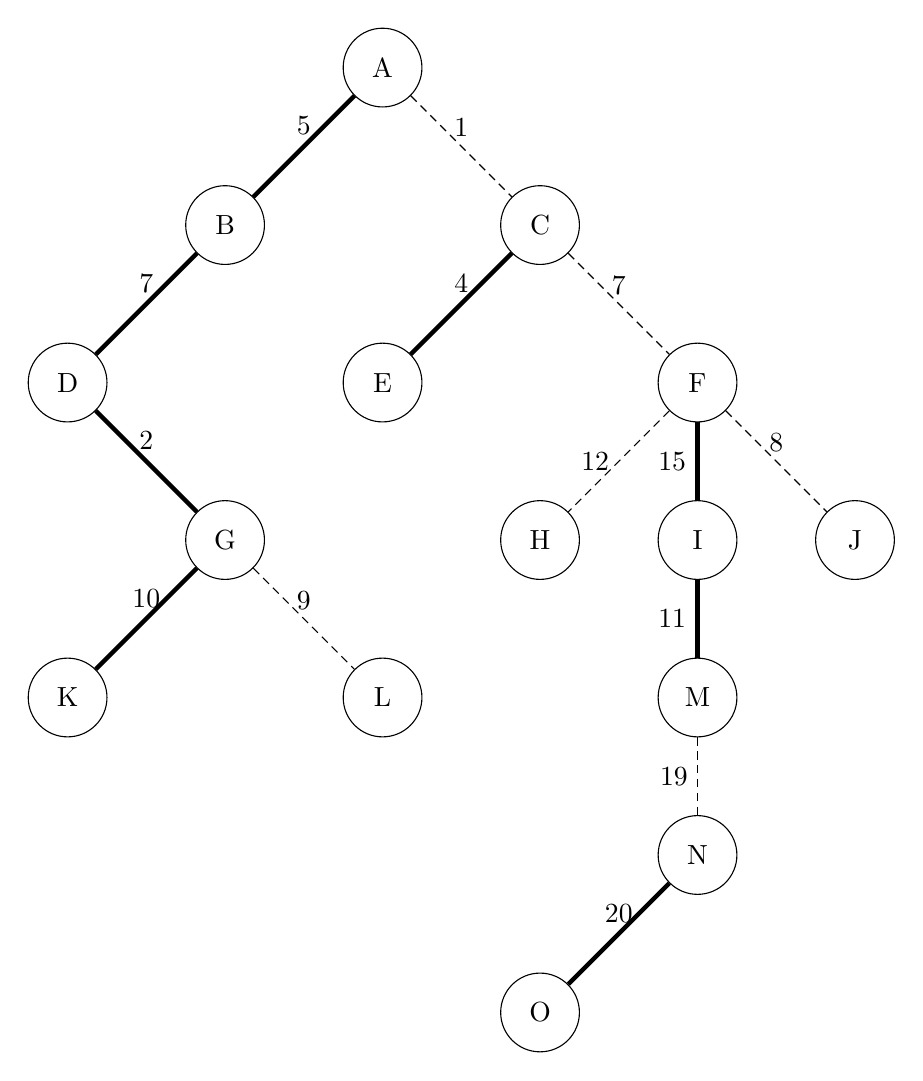
\begin{tikzpicture}[
            nointerno/.style={shape=circle, draw=black, minimum size=1cm},
            pref/.style={ultra thick},
            pptr/.style={densely dashed},
        ]
        \node[nointerno] (a) at (6, 20) {A};
        \node[nointerno] (b) at (4, 18) {B};
        \node[nointerno] (c) at (8, 18) {C};
        \node[nointerno] (d) at (2, 16) {D};
        \node[nointerno] (e) at (6, 16) {E};
        \node[nointerno] (f) at (10, 16) {F};
        \node[nointerno] (g) at (4, 14) {G};
        \node[nointerno] (h) at (8, 14) {H};
        \node[nointerno] (i) at (10, 14) {I};
        \node[nointerno] (j) at (12, 14) {J};
        \node[nointerno] (k) at (2, 12) {K};
        \node[nointerno] (l) at (6, 12) {L};
        \node[nointerno] (m) at (10, 12) {M};
        \node[nointerno] (n) at (10, 10) {N};
        \node[nointerno] (o) at (8, 8) {O};

        \draw[pref] (a) -- (b) node[midway, above] {5};
        \draw[pptr] (a) -- (c) node[midway, above] {1};
        \draw[pref] (b) -- (d) node[midway, above] {7};
        \draw[pref] (d) -- (g) node[midway, above] {2};
        \draw[pref] (g) -- (k) node[midway, above] {10};
        \draw[pptr] (g) -- (l) node[midway, above] {9};
        \draw[pptr] (c) -- (f) node[midway, above] {7};
        \draw[pref] (c) -- (e) node[midway, above] {4};
        \draw[pptr] (f) -- (h) node[midway, left] {12};
        \draw[pref] (f) -- (i) node[midway, left] {15};
        \draw[pptr] (f) -- (j) node[midway, above] {8};
        \draw[pref] (i) -- (m) node[midway, left] {11};
        \draw[pptr] (m) -- (n) node[midway, left] {19};
        \draw[pref] (n) -- (o) node[midway, above] {20};

    \end{tikzpicture}
    \caption{Árvore representada e seus caminhos preferidos. Na figura acima, as arestas escuras representam caminhos preferidos, com isso, temos o seguinte conjunto de caminhos vértice-disjuntos $ \{ \langle K,G,D,B,A \rangle, \langle E,C \rangle, \langle M,I,F \rangle, \langle L \rangle, \langle H \rangle, \langle J \rangle, \langle O,N \rangle \} $. }
    \label{fig:arvore-simples}
\end{figure}

%% ------------------------------------------------------------------------- %%
% access e como implementa o resto
\section{Operações}
\label{sec:lct-operacoes}

Nessa seção, apresentaremos o código por trás das operações que estamos interessados em implementar na link-cut tree. Em um primeiro momento, assumiremos que já sabemos como implementar alguns métodos que lidam com os caminhos preferidos. Desta forma, a implementação dos métodos abaixo fica reservada para a próxima seção.

\begin{itemize}
    \item \texttt{make\_identifier(u)}: transforma um vértice $u$ em identificador de seu caminho preferido.
    \item \texttt{split(u)}: recebe um nó $u$ e separa o caminho preferido que contém este nó em dois, quebrando a conexão entre $u$ e seu filho preferido, caso exista. Ao final, tanto $u$ quanto o seu filho preferido inicial serão os identificadores de seus caminhos.
    \item \texttt{join(u, v)}: recebe dois nós, $u$ e $v$ --- identificadores de seus caminhos e sendo $v$ um filho de $u$ na árvore representada --- e concatena os respectivos caminhos preferidos, transformando $uv$ em aresta preferida. Com isso, separa $u$ da parte mais profunda de seu caminho preferido inicial, deixando o identificador de tal caminho com um ponteiro para $u$. Ao final da operação, $u$ será o identificador do novo caminho criado.
    \item \texttt{reverse\_path(u)}: recebe $u$, o identificador de um caminho preferido, e inverte a orientação desse caminho, isto é, o fim se transforma no começo e o começo no fim.
    \item \texttt{get\_path\_end\_node(u)}: retorna o vértice menos profundo do caminho preferido de $u$, em outras palavras, o vértice no fim do caminho preferido que contém $u$. Na árvore da figura \ref{fig:arvore-simples}, a chamada \texttt{get\_path\_end\_node(G)} retorna o vértice \texttt{A}.
    \item \texttt{get\_parent\_path\_node(u)}: retorna o vértice ma floresta imediatamente acima do fim do caminho preferido que contém $u$; caso tal caminho contenha a raiz da árvore representada, este método retorna \texttt{null}. Aqui, na árvore da figura \ref{fig:arvore-simples}, \texttt{get\_parent\_path\_node(M)} retorna o vértice \texttt{C}.
    \item \texttt{get\_maximum\_path\_value(u)}: recebe $u$, o identificador de um caminho preferido, e retorna o maior valor de uma aresta neste caminho.
\end{itemize}

Com tal conjunto de funções, podemos avançar para os métodos da link-cut tree.

\subsection{Rotina Access}
\label{subsection:lct-access}

Uma rotina utilizada por todos os métodos da link-cut tree que vamos implementar é a \texttt{access(u)}, a partir dela conseguimos reorganizar a estrutura interna da árvore representada a nosso favor. Basicamente, a operação \texttt{access(u)} cria um caminho preferido que parte da raiz da árvore representada e vai até $u$. Com isso, todas as arestas preferidas que tinham somente uma das pontas fazendo parte deste novo caminho são destruídas e $u$ termina sem nenhum filho preferido.

Para isso, começamos uma sequência de iterações, que vão crescendo um caminho preferido desde $u$ até que tal caminho contemple a raiz da árvore representada. A cada iteração, fazemos com que uma variável \texttt{current\_root}, que inicialmente corresponde ao vértice $u$, vire o identificador de seu caminho preferido. Além disso, mantemos uma variável \texttt{last}, que corresponde a \texttt{current\_root} da iteração anterior, no início com valor igual a \texttt{null}.

Com estes valores em mãos, podemos ir criando um caminho preferido através de sucessivas concatenações, unindo o caminho que \texttt{current\_root} identifica a parte superior do caminho mantido por \texttt{last}. Ao final dessa concatenação, temos que \texttt{current\_root} é o identificador deste caminho que esta sendo construído, e após guardarmos seu valor em \texttt{last}, podemos prosseguir para o próximo passo, onde \texttt{current\_root} agora corresponde ao no imediatamente em cima do caminho preferido que estamos construindo.

\begin{algorithm}[h!]
    \caption{Access}\label{lct:access}
    \begin{algorithmic}
        \Function{access}{$u$}
        \State $last \gets NULL$
        \State $current\_root \gets u$
        \State \Comment{concatena todos os caminhos preferidos de $u$ até a raiz da árvore representada}
        \While{$current\_root \neq NULL$}
        \State $make\_identifier(current\_root)$
        \State \Comment{concatena um novo pedaço de caminho preferido ao caminho em que \texttt{last} é identificador}
        \State $join(current\_root, last)$
        \State $last \gets current\_root$
        \State $current\_root \gets get\_parent\_path\_node(current\_root)$
        \State $make\_identifier(u)$
        \EndWhile
        \EndFunction
    \end{algorithmic}
\end{algorithm}

Ao final da iteração, colocamos o vértice $u$ como identificador deste novo caminho preferencial, simplificando as operações a seguir.

\begin{figure}
    \centering
    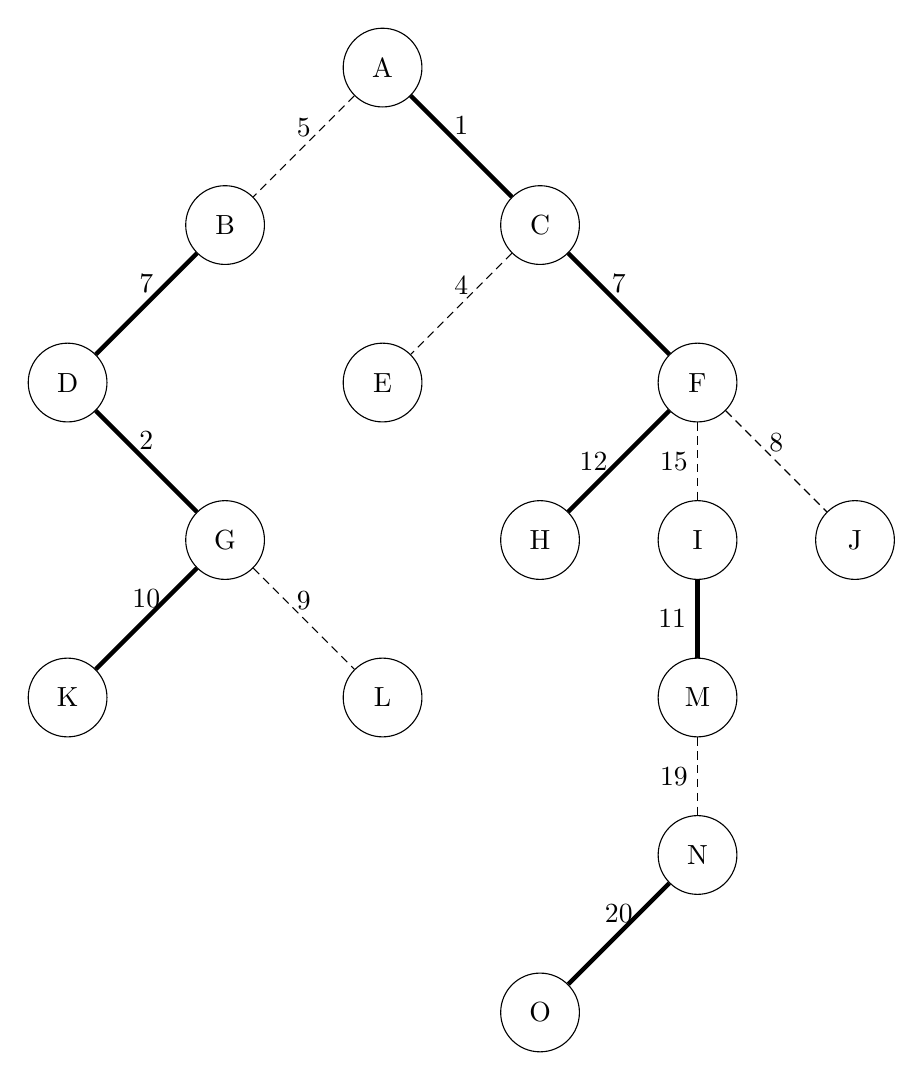
\begin{tikzpicture}[
            nointerno/.style={shape=circle, draw=black, minimum size=1cm},
            pref/.style={ultra thick},
            pptr/.style={densely dashed},
        ]
        \node[nointerno] (a) at (6, 20) {A};
        \node[nointerno] (b) at (4, 18) {B};
        \node[nointerno] (c) at (8, 18) {C};
        \node[nointerno] (d) at (2, 16) {D};
        \node[nointerno] (e) at (6, 16) {E};
        \node[nointerno] (f) at (10, 16) {F};
        \node[nointerno] (g) at (4, 14) {G};
        \node[nointerno] (h) at (8, 14) {H};
        \node[nointerno] (i) at (10, 14) {I};
        \node[nointerno] (j) at (12, 14) {J};
        \node[nointerno] (k) at (2, 12) {K};
        \node[nointerno] (l) at (6, 12) {L};
        \node[nointerno] (m) at (10, 12) {M};
        \node[nointerno] (n) at (10, 10) {N};
        \node[nointerno] (o) at (8, 8) {O};

        \draw[pptr] (a) -- (b) node[midway, above] {5};
        \draw[pref] (a) -- (c) node[midway, above] {1};
        \draw[pref] (b) -- (d) node[midway, above] {7};
        \draw[pref] (d) -- (g) node[midway, above] {2};
        \draw[pref] (g) -- (k) node[midway, above] {10};
        \draw[pptr] (g) -- (l) node[midway, above] {9};
        \draw[pref] (c) -- (f) node[midway, above] {7};
        \draw[pptr] (c) -- (e) node[midway, above] {4};
        \draw[pref] (f) -- (h) node[midway, left] {12};
        \draw[pptr] (f) -- (i) node[midway, left] {15};
        \draw[pptr] (f) -- (j) node[midway, above] {8};
        \draw[pref] (i) -- (m) node[midway, left] {11};
        \draw[pptr] (m) -- (n) node[midway, left] {19};
        \draw[pref] (n) -- (o) node[midway, above] {20};

    \end{tikzpicture}
    \caption{Caminhos preferidos na árvore da figura \ref{fig:arvore-simples} após uma operação de \texttt{access} no nó $H$. Com isso temos o novo conjunto de caminhos vértice-disjuntos $ \{ \langle H,F,C,A \rangle, \langle K,G,D,B \rangle, \langle M,I \rangle, \langle E \rangle, \langle J \rangle, \langle L \rangle, \langle O,N \rangle \} $. }
    \label{fig:arvore-access}
\end{figure}

\subsection{Rotinas Make Root, Link e Cut}
\label{subsection:lct-make-root}

Em seguida, temos a função \texttt{make\_root(u)}, que enraíza em $u$ a árvore representada que o contém. Para isso, criamos um caminho preferencial que vai da raiz da árvore ate $u$, utilizando \texttt{access(u)}. Em seguida, utilizamos a rotina \texttt{reverse\_path(u)}, que inverte a orientação deste caminho preferido recém-criado. Tal inversão coloca $u$ como o vértice de menor profundidade da árvore representada, o que se traduz neste sendo a nova raiz.

\begin{algorithm}[h!]
    \caption{Make Root}\label{lct:make-root}
    \begin{algorithmic}
        \Function{make\_root}{$u$}
        \State $access(u)$
        \State $reverse\_path(u)$
        \EndFunction
    \end{algorithmic}
\end{algorithm}

Como rotinas que dão nome a nossa estrutura, temos \texttt{link(u, v, w)} e \texttt{cut{u, v}}.

A primeiro delas, recebe dois vértices $u$ e $v$ que estão em árvores distintas, e cria uma aresta de peso $w$, conectando-os. Primeiramente, devemos lembrar que as arestas da árvore representada viram vértices em nossa representação interna. Com isso, o primeiro passo é criar um vértice que tem seu valor definido como $w$, vamos chama-lo \texttt{uv\_edge}. Dessa forma, criaremos as seguintes conexões: $u \leftrightarrow uv\_edge \leftrightarrow v$.

Inicialmente, colocamos $v$ como raiz de nossa árvore representada, e criamos um caminho preferido que só possui este vértice como integrante. Com isso, conseguimos concatenar este caminho preferido de tamanho unitário com o caminho que \texttt{uv\_edge} constitui. A seguir, aplicamos a mesma ideia, criando um caminho unitário que contém $u$ e o concatenando com um caminho que possui $v$ e \texttt{uv\_edge}.

\begin{algorithm}[h!]
    \caption{Link}\label{lct:link}
    \begin{algorithmic}
        \Require{$u$ e $v$ em árvores distintas}
        \Function{link}{$u, v, w$}
        \State $uv\_edge := new Node(w)$ \Comment{cria nó com peso $w$, representando a aresta}
        \State \Comment{ligando $(v) - (uv\_edge)$}
        \State $make\_root(v)$
        \State $access(v)$
        \State $join(v, uv\_edge)$
        \State \Comment{ligando $(uv\_edge)-(u)$}
        \State $make\_root(u);$
        \State $access(u)$
        \State $access(uv\_edge)$
        \State $join(uv\_edge, u)$
        \EndFunction
    \end{algorithmic}
\end{algorithm}

Já a operação \texttt{cut(u, v)}, que separa dois nós, é um pouco mais simples. Note que, temos que separar as conexões entre $u$ e \texttt{uv\_edge} assim como entre \texttt{uv\_edge} e $v$. O processo de separação é igual para as duas partes, por isso, vamos explicar somente a separação de $u$ e \texttt{uv\_edge}.

A ideia é colocarmos $u$ como raiz de nossa árvore representada, com isso, podemos criar um caminho preferido vai de $u$ até $u$ e \texttt{uv\_edge}. Agora, basta usarmos nossa operação $u$ e \texttt{split(uv\_edge)}, que separa \texttt{uv\_edge} da parte superior de seu caminho preferido, efetivamente quebrando sua conexão com $u$.

\begin{algorithm}[h!]
    \caption{Cut}\label{lct:cut}
    \begin{algorithmic}
        \Require{$u$ e $v$ na mesma árvore}
        \Function{cut}{$u, v$}
        \State \Comment{cortando $(u) - (uv\_edge)$}
        \State $make\_root(u)$
        \State $access(uv\_edge)$
        \State $split(uv\_edge)$
        \State \Comment{cortando $(v) - (uv\_edge)$}
        \State $make\_root(v)$
        \State $access(uv\_edge)$
        \State $split(uv\_edge)$
        \EndFunction
    \end{algorithmic}
\end{algorithm}

\subsection{Consultas Is Connected e Maximum Edge}
\label{subsection:lct-is-connected}

A função \texttt{is\_connected(u, v)}, que nos informa se $u$ e $v$ pertencem a mesma árvore, funciona da seguinte maneira. Primeiro acessamos $u$, criando um caminho deste até a raiz da árvore. Em seguida, guardamos o vértice que esta no fim desse caminho, isto é, guardamos a raiz da árvore que contém $u$. A seguir, repetimos o mesmo processo com o vértice $v$. Agora, basta compararmos se ambos os valores que guardamos são iguais.

\begin{algorithm}[h!]
    \caption{Is Connected}\label{lct:is-connected}
    \begin{algorithmic}
        \Function{is\_connected}{$u, v$}
        \State $access(u)$
        \State $u\_tree\_root \gets get\_path\_end\_node(u)$
        \State $access(v)$
        \State $v\_tree\_root \gets get\_path\_end\_node(v)$
        \State \Return $(u\_tree\_root = v\_tree\_root)$
        \EndFunction
    \end{algorithmic}
\end{algorithm}

Por último, temos a função \texttt{maximum\_edge(u, v)}, que retorna o peso da maior aresta no caminho simples entre $u$ e $v$. Como transformamos as arestas em vértices na nossa representação interna, precisamos procurar o maior valor de um vértice no caminho preferido entre $u$ e $v$. Para isso, transformamos $v$ na raiz de nossa árvore e acessamos $u$. Com isso, podemos utilizar \texttt{get\_maximum\_path\_value(u)} para obter o maior valor contido neste caminho preferido.

\begin{algorithm}[h!]
    \caption{Maximum Edge}\label{lct:max-edge}
    \begin{algorithmic}
        \Require{$u$ e $v$ na mesma árvore}
        \Function{maximum\_edge}{$u, v$}
        \State $make\_root(v)$
        \State $access(u)$
        \State \Return $get\_maximum\_path\_value(u)$
        \EndFunction
    \end{algorithmic}
\end{algorithm}

E com isso, encerramos a explicação da implementação dos métodos da link-cut tree.

%% ------------------------------------------------------------------------- %%
%% ------------------------------------------------------------------------- %%
%% ------------------------------------------------------------------------- %%
%% ------------------------------------------------------------------------- %%
\section{Splay Tree}
\label{sec:lct-splay-trees}

No artigo original, Sleator e Tarjan propuseram a utilização de uma árvore binária enviesada como estrutura para os caminhos preferidos. Porém, quatro anos depois, eles apresentaram a splay tree ~\citep{10.1145/3828.3835}, que possibilita realizarmos as operações necessárias para a manipulação dos caminhos preferidos em tempo $\Oh(\log n)$ amortizado, com uma implementação muito mais limpa do que a da versão original. Portanto, usaremos a splay trees para armazenar os caminhos preferidos.

Uma splay tree é uma árvore binária de busca auto-balanceável. Estas árvores utilizam rotações para auto-balancear, através de uma operação chamada \texttt{splay}. A operação \texttt{splay}, traz um nó para a raiz da árvore através de sucessivas rotações. Mas antes de nos aprofundarmos neste método, examinaremos como os caminhos preferidos são representados aqui.

Primeiramente, em nosso uso, a ordenação dos nós na splay tree é dada pela profundidade destes na link-cut tree. Note que não guardamos explicitamente esses valores. Em vez disso, utilizamos a ideia de chave implícita, isto é, só nos preocupamos em manter a ordem relativa dos nós após as operações de separação e união das árvores, apresentadas a seguir. Em contrapartida, com este método, perdemos a capacidade de realizarmos buscas por chave na splay tree, porém não necessitamos dessa operação.

Ademais, para implementar eficientemente a operação \texttt{get\_maximum\_path\_value}, mantemos o peso máximo dos nós em cada sub-árvore de uma splay tree.

\begin{figure}
    \centering
    \begin{tikzpicture}[
            no/.style={shape=circle, draw=black, minimum size=1cm},
            novertice/.style={shape=rectangle, draw=black, minimum size=1cm},
            aresta/.style={thick},
        ]
        \node[no] (f) at (6, 10) {F};
        \node[novertice] (ac) at (4, 8) {\shortstack{AC\\$1$}};
        \node[novertice] (fh) at (8, 8) {\shortstack{FH\\$12$}};
        \node[no] (a) at (2, 6) {A};
        \node[no] (c) at (6, 6) {C};
        \node[no] (h) at (10, 6) {H};
        \node[novertice] (cf) at (4, 4) {\shortstack{CF\\$7$}};

        \draw[aresta] (f) -- (ac);
        \draw[aresta] (f) -- (fh);
        \draw[aresta] (ac) -- (a);
        \draw[aresta] (ac) -- (c);
        \draw[aresta] (a) -- (cf);
        \draw[aresta] (fh) -- (h);

    \end{tikzpicture}
    \caption{Uma possível configuração da splay tree que armazena o caminho preferido $\langle H,F,C,A \rangle$ da figura \ref{fig:arvore-access}, onde $F$ é identificador do caminho. Os nós em formato retangular mostram as arestas da árvore representada, com o peso de tal aresta na parte inferior.}
    \label{fig:splay-path}
\end{figure}

Além disso, como usamos a profundidade dos nós na árvore representada como chave para a árvore auxiliar, temos que todos os nós na sub-árvore esquerda da raiz de uma splay tree têm uma profundidade menor que a raiz, enquanto os nós à direita têm uma profundidade maior. Contudo, ao realizamos uma operação \texttt{make\_root(u)}, fazemos com que todos os nós que estavam acima de $u$ na árvore representada se tornem parte de sua sub-árvore. Para isso, incluímos na splay tree um mecanismo para inverter a ordem de todos os nós de uma árvore auxiliar, efetivamente invertendo a orientação de um caminho preferido.

Com isso, os nós da árvore auxiliar têm os seguintes campos:

\begin{itemize}
    \item \texttt{parent}: apontador para o pai na splay tree. Caso o nó em particular seja a raiz da árvore auxiliar, este campo armazena um ponteiro para o vértice que está logo acima do fim deste caminho preferido na árvore representada.
    \item \texttt{left\_child} e \texttt{right\_child}: apontadores para os filhos esquerdo e direito de um nó na splay tree.
    \item \texttt{value}: se o nó representa uma aresta da árvore representada guarda o peso desta aresta, senão guarda 0.
    \item \texttt{is\_reversed}: valor booleano para sinalizar se a sub-árvore do nó esta com sua ordem invertida ou não, isto é, se todas as posições de filhos esquerdos e direitos estão  invertidas nessa  sub-árvore.
    \item \texttt{max\_subtree\_value}: guarda o valor máximo armazenado na sub-árvore do nó.
\end{itemize}

\subsection{Splay}
\label{subsection:lct-splay-splay}

Com a estrutura apresentada, podemos partir para a explicação de sua principal operação, a \texttt{splay}. Em poucas palavras, este método é responsável por receber um nó e fazer com que ele vire a raiz da splay tree, através de diversas rotações.  Ademais, as operações de \texttt{splay} contribuem para diminuir a altura da árvore, melhorando o seu consumo de tempo.

Em particular, podemos dizer que esta operação é responsável por transformar um vértice em identificador de seu caminho, ou seja, entendemos como sinônimos os métodos \texttt{make\_identifier} e \texttt{splay}.

De modo a facilitarmos nossa explicação, chamamos \texttt{parent} o pai de um nó $u$ e de \texttt{grandparent} o pai de \texttt{parent}.

Primeiramente, uma operação de \texttt{splay} consiste em realizamos diversos passos de \emph{splay}, que trazem $u$ cada vez mais próximo à raiz da árvore, isto é, em cada um desses passos, realizamos uma rotação que diminui a profundidade de $u$. Porém, ao realizar estes passos, temos que nos preocupar com dois fatores:

\begin{itemize}
    \item A propagação do valor booleano $is\_reversed$ de \texttt{grandparent} e em seguida o de \texttt{parent}, fazendo as devidas reversões caso necessárias. Isso nos fornece a invariante de que iremos fazer comparações entre os filhos corretos para determinar qual rotação fazer.
    \item A orientação que \texttt{grandparent}, \texttt{parent} e $u$ se encontram, isto é, se estão em uma orientação de \textit{zig}, \textit{zig-zig} ou \textit{zig-zag}, como exemplificadas na figura \ref{fig:zig-oris}. Dependendo da orientação, fazemos uma rotação em $u$ ou em \texttt{parent}, sempre com a ideia de diminuirmos em 1 a profundidade de $u$.
\end{itemize}

\begin{figure}
    \centering
    \begin{subfigure}[b]{0.3\textwidth}
        \centering
        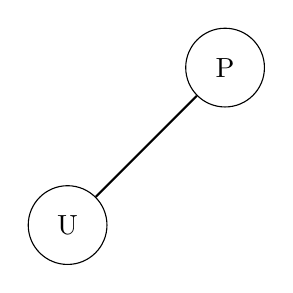
\begin{tikzpicture}[
                no/.style={shape=circle, draw=black, minimum size=1cm},
                aresta/.style={thick},
            ]
            \node[no] (u) at (0, 0) {U};
            \node[no] (p) at (2, 2) {P};
            \draw[aresta] (u) -- (p);
        \end{tikzpicture}
        \caption{zig}
    \end{subfigure}
    \hfill
    \begin{subfigure}[b]{0.3\textwidth}
        \centering
        \begin{tikzpicture}[
                no/.style={shape=circle, draw=black, minimum size=1cm},
                aresta/.style={thick},
            ]
            \node[no] (u) at (0, 0) {U};
            \node[no] (p) at (2, 2) {P};
            \node[no] (gp) at (4, 4) {GP};
            \draw[aresta] (u) -- (p);
            \draw[aresta] (p) -- (gp);
        \end{tikzpicture}
        \caption{zig-zig}
    \end{subfigure}
    \hfill
    \begin{subfigure}[b]{0.3\textwidth}
        \centering
        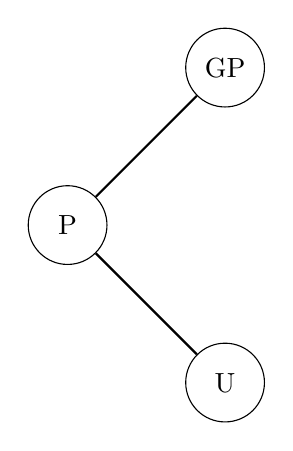
\begin{tikzpicture}[
                no/.style={shape=circle, draw=black, minimum size=1cm},
                aresta/.style={thick},
            ]
            \node[no] (u) at (4, 0) {U};
            \node[no] (p) at (2, 2) {P};
            \node[no] (gp) at (4, 4) {GP};
            \draw[aresta] (u) -- (p);
            \draw[aresta] (p) -- (gp);
        \end{tikzpicture}
        \caption{zig-zag}
    \end{subfigure}
    \caption{Orientações \textit{zig}, \textit{zig-zig} e \textit{zig-zag} na splay tree. Aqui, \texttt{P} e \texttt{GP} abreviam \texttt{parent} e \texttt{grandparent}, respectivamente.}
    \label{fig:zig-oris}
\end{figure}


Ao sair da função \texttt{splay}, o nó $u$ estará na raiz de sua árvore auxiliar. Além disso, seu valor booleano $is\_reversed$ estará nulo, pois as reversões já terão sido propagadas aos seus filhos, e seu $max\_subtree\_value$ estará atualizado, contendo o maior valor presente na splay tree.

\begin{algorithm}[h!]
    \caption{splay}\label{splay:splay}
    \begin{algorithmic}
        \Function{Splay}{$u$}
        \While{$!u.is\_root()$} \Comment{$u$ não ser raiz da LCT e nem da Splay}
        \State $parent \gets u.parent$
        \State $grandparent \gets parent.parent$
        \If{$!parent.is\_root()$}
        % \State \Comment{propagamos o \texttt{is\_reversed} bit do \texttt{grandparent} para o \texttt{parent} para garantir que a condicional a seguir usa os filhos corretos para a comparação}
        \State $grandparent.push_reversed_bit()$
        \State $parent.push\_reversed\_bit()$
        \If{$(grandparent.r\_child = parent) = (parent.r\_child = u)$}
        \State $rotate(parent)$\Comment{zig-zig ou zag-zag}
        \Else
        \State $rotate(u)$\Comment{zig-zag}
        \EndIf
        \EndIf
        \State $rotate(u)$
        \EndWhile
        \State $u.push\_reversed\_bit()$
        \EndFunction
    \end{algorithmic}
\end{algorithm}

Assim como a operação acima, o restante da nossa implementação de uma splay tree é bastante tradicional. Com isso, nossos únicos cuidados extras são a manutenção do bit \texttt{is\_reversed}, do valor máximo das sub-árvores e da manutenção das chaves implícitas. Assim, no método \texttt{rotate(u)}, temos como primeiro passo a propagação do bit \texttt{is\_reversed} de \texttt{grandparent} até $u$ e como última etapa o cálculo dos novos valores de \texttt{max\_subtree\_value}.

\subsection{Split e Join}
\label{subsection:lct-splay-split-join}

Temos também dois métodos importantes das splay trees usados na manutenção dos caminhos preferidos, \texttt{split} e \texttt{join}, responsáveis por separar e concatenar caminhos preferidos, respectivamente.

\begin{algorithm}[h!]
    \caption{Split}\label{splay:split}
    \begin{algorithmic}
        \Function{split}{$u$}
        \If{$u.l\_child \neq NULL$}
        \State $u.l\_child.parent \gets NULL$
        \EndIf
        \State $u.l\_child \gets NULL$
        \EndFunction
    \end{algorithmic}
\end{algorithm}

Primeiramente, falaremos do método \texttt{split(u)}, que recebe um nó $u$ e separa caminho preferido que o contem em dois. Para isso, ele simplesmente separa a sub-árvore esquerda de $u$, como mostrado acima. Vale notar que, este método é destrutivo: removendo tanto o ponteiro para o filho preferido de $u$ quanto o ponteiro \texttt{parent} que tal filho possui para $u$. Logo, usamos essa rotina apenas para o \texttt{cut()} da link-cut tree.

\begin{algorithm}[h!]
    \caption{Join}\label{splay:join}
    \begin{algorithmic}
        \Require{$u$ e $v$ identificadores de seus caminhos preferidos}
        \Function{join}{$u, v$}
        \If{$v \neq NULL$}
        \State $v.parent \gets u$
        \EndIf
        \State $u.r\_child \gets v$
        \State \Comment{atualiza \texttt{max\_subtree\_value} com o máximo entre o \texttt{value} dos dois filhos de $u$}
        \State $u.recalculate\_max\_subtree\_value()$
        \EndFunction
    \end{algorithmic}
\end{algorithm}

De maneira complementar, temos a rotina \texttt{join(u, v)} que recebe dois nós e concatena os respectivos caminhos preferidos. Para isso, assume-se que ambos os nós sejam identificadores de seus caminhos preferidos, ou seja, que eles sejam as raízes de suas splay trees. Com isso, simplesmente colocamos a splay tree em que $v$ é raiz como a sub-árvore direita de $u$, atualizando os respetivos apontadores e recalculando o valor máximo na splay tree de $u$. Note que, a sub-árvore direita inicial, que constitui a parte do caminho preferido de $u$ que foi substituída, ficará com um apontador \texttt{parent} para $u$.

\subsection{Métodos auxiliares}
\label{subsection:lct-splay-aux}

Para finalizar, nossa splay tree possui quatro métodos auxiliares, o \texttt{reverse\_path}, \texttt{get\_path\_end\_node}, \texttt{get\_parent\_path\_node} e \texttt{get\_maximum\_path\_value}.

\begin{algorithm}[h!]
    \caption{Revese Path}\label{splay:reverse-path}
    \begin{algorithmic}
        \Require{$u$ identificador de seu caminho preferido}
        \Function{revese\_path}{$u$}
        \State $u.is\_reversed \gets !u.is\_reversed$
        \State $u.push\_reversed\_bit()$ \Comment{inverte os filhos de $u$ e propaga a inversão do bit}
        \EndFunction
    \end{algorithmic}
\end{algorithm}

Primeiramente, o \texttt{reverse\_path(u)} recebe o identificador de um caminho e inverte a orientação desse caminho. Tal tarefa é realizada invertendo o valor do bit \texttt{is\_reversed} de $u$, com isso, nas próximas operações realizadas neste nó, seus filhos serão trocados de posição e o bit sera propagado na sub-árvore.

\begin{algorithm}[h!]
    \caption{Get Path End Node}\label{splay:get-path-end}
    \begin{algorithmic}
        \Function{get\_path\_end\_node}{$u$}
        \State $splay(u)$
        \State $smallest\_value \gets u$
        \While{$smallest\_value.l\_child \neq NULL$}
        \State $smallest\_value \gets smallest\_value.l\_child$
        \EndWhile
        \State $splay(smallest\_value)$ \Comment{garantido que sera mais rápido na próxima vez}
        \State \Return $smallest\_value$
        \EndFunction
    \end{algorithmic}
\end{algorithm}

\begin{algorithm}[h!]
    \caption{Get Parent Path Node}\label{splay:get-parent-path}
    \begin{algorithmic}
        \Function{get\_parent\_path\_node}{$u$}
        \State $splay(u)$
        \State \Return $u.parent$
        \EndFunction
    \end{algorithmic}
\end{algorithm}

A seguir, os métodos \texttt{get\_path\_end\_node(u)} e \texttt{get\_parent\_path\_node(u)} são usados para acessar o fim e o pai do caminho preferido que contem $u$. Em particular, a primeira rotina retorna o vértice menos profundo do caminho preferido de $u$, fazendo isso ao acessar o vértice mais à esquerda na splay tree. Já o segundo método é responsável por retornar o vértice imediatamente acima do fim do caminho preferido que contêm $u$, caso tal caminho contenha a raiz da árvore representada, este método retorna \texttt{null}. Para fazer isso, efetuamos uma operação \texttt{splay} em $u$ e retornamos o valor de \texttt{parent}.

\begin{algorithm}[h!]
    \caption{Get Maximum Path Value}\label{splay:get-maximum-value}
    \begin{algorithmic}
        \Require{$u$ identificador de seu caminho preferido}
        \Function{get\_maximum\_path\_value}{$u$}
        \State \Return $u.max\_subtree\_value$
        \EndFunction
    \end{algorithmic}
\end{algorithm}

Por último, temos a função \texttt{get\_maximum\_path\_value(u)}, que recebe um vértice identificador de caminho $u$ e retorna o maior valor de uma aresta no caminho preferencial de $u$, em termos práticos, retorna o valor de \texttt{max\_subtree\_value}.

Com isso, temos todas as ferramentas necessárias para manipularmos a splay tree em seu uso como árvore auxiliar.